%%=============================================================================
%DIF LATEXDIFF DIFFERENCE FILE
%DIF DEL /scratch/seaver/tmp/tmp.KDMsLKaKux/old/Papers/NAR_Update_2026/latex/main.tex   Thu Oct  1 20:01:45 2026
%DIF ADD /scratch/seaver/tmp/tmp.KDMsLKaKux/new/Papers/NAR_Update_2026/latex/main.tex   Fri Oct  2 16:11:24 2026
%%  The ModelSEED Biochemistry Database: 2026 update
%%  Target journal: Nucleic Acids Research (NAR), Database Issue
%%  https://academic.oup.com/nar/pages/Ms_Prep_Database
%%
%%  This is the ONLY file that carries journal formatting. All prose lives in
%%  sections/ and is pulled in by the \input statements at the bottom.
%%  Build:  pdflatex main -> bibtex main -> pdflatex main -> pdflatex main
%%          (or simply: latexmk -pdf main.tex)
%%=============================================================================

%%-----------------------------------------------------------------------------
%%  NAR DATABASE-ISSUE REQUIREMENTS CHECKLIST
%%  Summary only. The authoritative, fully-cited version -- including OUP's
%%  figure format/dpi specification -- is in NAR_REQUIREMENTS.md alongside
%%  this file. Update that file, not this comment.
%%  (from academic.oup.com/nar/pages/Ms_Prep_Database, checked 2026-08-26)
%%
%%  [ ] LENGTH -- update papers: normally no more than 4-6 typeset journal
%%      pages. Contact the Executive Editor before submitting anything longer.
%%      Current draft is deliberately over; trim after [TBD] markers resolve.
%%  [!] TITLE -- the database name should ideally be the FIRST WORD of the
%%      title. Current title opens with "The". Consider "ModelSEED Biochemistry
%%      Database, 2026 update: ..." to comply.
%%  [ ] URL -- a working URL must appear BOTH in the abstract and in the body.
%%      See \modelseedurl below; used in the abstract. The body carries the
%%      repository URL in sections/data_availability.tex.
%%  [ ] GRAPHICAL ABSTRACT -- MANDATORY. 5:2 aspect ratio, min 127x50 mm
%%      (5x2 in), TIF/EPS/editable PDF, 300-600 dpi, landscape, sans-serif
%%      (Arial) 12-16 pt. Must be ORIGINAL -- not reused from any main or
%%      supplementary figure. No trademarked/copyrighted logos.
%%      Submitted as a separate file, not embedded here.
%%  [ ] REFERENCES -- numbered sequentially in order of appearance. The class
%%      default (no namedate/numbered option) gives NAR-style numeric (1,2).
%%      Exclude "submitted"/"in preparation"/personal communications.
%%      Cite other databases by their most recent published description; if
%%      none exists, put the URL in body text, NOT in the reference list.
%%  [ ] FIGURES -- no numeric limit on figure count; the 4-6 page budget is the
%%      real constraint. The database home page may NOT be used as a typeset
%%      figure. A representative screenshot of a query result IS allowed.
%%      Format (OUP artwork guidance): raster -> uncompressed .tif; vector ->
%%      .eps/.svg/.pdf with embedded fonts. Minimum dpi: 300 colour half-tone,
%%      600 greyscale, 600-900 combination/line art, 1200 mono line art; vector
%%      has no inherent resolution. RGB preferred. Arial/Times/Courier/Symbol,
%%      text >= 7pt, lines 0.25-1pt. Prefer vector PDF/EPS from the figure
%%      scripts -- it sidesteps the dpi table entirely. See NAR_REQUIREMENTS.md.
%%  [ ] DATA AVAILABILITY -- must address formats and terms for data download.
%%  [ ] DATABASE ACCESS -- must be freely accessible without login; HTTPS
%%      encouraged; URL persistence expected for >= 5 years post-publication.
%%      Mobile/tablet accessibility is worth mentioning explicitly.
%%  [ ] INITIAL SUBMISSION -- one .pdf with main text, references, tables and
%%      figures EMBEDDED. Supplementary data as separate file(s). Number all
%%      pages (the class does this). Single-column/single-spaced is waived for
%%      LaTeX, so the two-column class output is correct as-is.
%%      DO NOT use line-numbering. DO NOT use footnotes. (Verified absent.)
%%  [ ] DISCLOSURES -- ORCID REQUIRED for the submitting author. Author
%%      Contributions statement MANDATORY (CRediT encouraged). Conflict of
%%      interest disclosure REQUIRED. AI assistance used in preparing this
%%      manuscript MUST be disclosed in the cover letter and in Methods or
%%      Acknowledgements. See NAR_REQUIREMENTS.md section 13.
%%  [ ] CODE DEPOSIT -- a GitHub URL is not sufficient; deposit to Zenodo or
%%      FigShare and put the permanent DOI in Data Availability at revision.
%%  [ ] SUBMISSION -- at least six suggested referees (name, institute, email),
%%      independent, not same institution/city as any author. Handled in
%%      ScholarOne at submission time, not in this file.
%%  [ ] DEADLINE -- update manuscripts due 15 September. Nothing before 1 June.
%%-----------------------------------------------------------------------------

%% NAR specifies the OUP template's "Modern Large" design -- do not change these
%% two options without checking NAR_REQUIREMENTS.md section 7 first.
%% Modern/large gives: 9bp body on 11.5pt leading, SANS-SERIF body text
%% (modern is the only one of the three designs that forces \sffamily),
%% 7.5bp footnotes, 210x276mm paper, two columns.
%% Other designs exist (contemporary|traditional x large|medium|mediumone|small)
%% but are not what NAR asks for.
%% Omitting namedate/numbered keeps the class default = numeric citations (NAR style).
\documentclass[unnumsec,webpdf,modern,large]{oup-authoring-template}

%\onecolumn  % uncomment for a wide single-column reading/review draft

%%-----------------------------------------------------------------------------
%DIF 82a82-88
%%  NAR revision markup: the referee-facing "marked" copy is now generated by %DIF > 
%%  running latexdiff between the pre-PR-297 and post-PR-297 versions of this %DIF > 
%%  file (see Papers/NAR_Update_2026/latex/README or the PR description for %DIF > 
%%  the exact command). No in-source markup macro is needed any more. %DIF > 
%%----------------------------------------------------------------------------- %DIF > 
 %DIF > 
%%----------------------------------------------------------------------------- %DIF > 
%DIF -------
%%  Packages. The class already loads: amsmath, amssymb, graphicx, hyperref,
%%  natbib, array, multirow, xcolor, tikz, url, caption, rotating, listings.
%%  It also defines \toprule / \midrule / \botrule itself -- do NOT load
%%  booktabs, it clashes.
%%-----------------------------------------------------------------------------
%% NOTE: the OUP manual asks authors to "refrain from adding further packages
%% or macros if possible", so nothing is loaded here. The draft-marker and
%% domain-shorthand macros below are the only additions, and the markers
%% disappear entirely under \draftmodefalse.

%%-----------------------------------------------------------------------------
%%  Draft markers.
%%  The source manuscript carries [TBD] and [DRAFT PENDING] placeholders.
%%  They are rendered in colour while drafting so they are impossible to miss.
%%  Flip \draftmodefalse (or pass \draftmodefalse before \begin{document})
%%  to make every marker vanish for a clean submission PDF.
%%-----------------------------------------------------------------------------
\newif\ifdraftmode
\draftmodetrue          % <-- set to \draftmodefalse for the submission build

\ifdraftmode
  \newcommand{\TBD}[1][]{\textcolor{red}{\textbf{[TBD}\ifx\relax#1\relax\else\ #1\fi\textbf{]}}}
  \newcommand{\DRAFTPENDING}[1]{\textcolor{orange}{\textbf{[DRAFT PENDING]}\ --\ #1}}
  \newcommand{\NUMBERSPENDING}[1]{\textcolor{orange}{\textbf{[NUMBERS PENDING]}\ #1}}
\else
  \newcommand{\TBD}[1][]{}
  \newcommand{\DRAFTPENDING}[1]{}
  \newcommand{\NUMBERSPENDING}[1]{}
\fi

%%-----------------------------------------------------------------------------
%%  Domain shorthands. Greek in text mode is unreliable under pdflatex, so all
%%  thermodynamic symbols route through math mode here.
%%-----------------------------------------------------------------------------
\newcommand{\dfG}{$\Delta_{\mathrm{f}}G'$}          % formation energy
\newcommand{\drG}{$\Delta_{\mathrm{r}}G'$}          % reaction energy
\newcommand{\drGo}{$\Delta_{\mathrm{r}}G'^{\circ}$} % standard reaction energy
\newcommand{\modelseedurl}{\url{https://modelseed.org}}
\newcommand{\repourl}{\url{https://github.com/ModelSEED/ModelSEEDDatabase}}
\newcommand{\file}[1]{\texttt{#1}}                  % repo paths / filenames
\newcommand{\cpd}[1]{\texttt{#1}}                   % compound identifiers

%% The OUP class sets \flushbottom (cls line 2513). With a short column the
%% slack is absorbed by the most elastic glue on the page -- the space above
%% \subsection headings -- which opened visible gaps before 'Atom mapping'
%% and 'Distribution and community process'. \raggedbottom lets a column end
%% short instead. Standard LaTeX, no package and no class option.
\raggedbottom
%DIF PREAMBLE EXTENSION ADDED BY LATEXDIFF
%DIF UNDERLINE PREAMBLE %DIF PREAMBLE
\RequirePackage[normalem]{ulem} %DIF PREAMBLE
\RequirePackage{color}\definecolor{RED}{rgb}{1,0,0}\definecolor{BLUE}{rgb}{0,0,1} %DIF PREAMBLE
\providecommand{\DIFadd}[1]{{\protect\color{red}\uwave{#1}}} %DIF PREAMBLE
\providecommand{\DIFdel}[1]{{\protect\color{blue}\sout{#1}}} %DIF PREAMBLE
%DIF SAFE PREAMBLE %DIF PREAMBLE
\providecommand{\DIFaddbegin}{} %DIF PREAMBLE
\providecommand{\DIFaddend}{} %DIF PREAMBLE
\providecommand{\DIFdelbegin}{} %DIF PREAMBLE
\providecommand{\DIFdelend}{} %DIF PREAMBLE
\providecommand{\DIFmodbegin}{} %DIF PREAMBLE
\providecommand{\DIFmodend}{} %DIF PREAMBLE
%DIF FLOATSAFE PREAMBLE %DIF PREAMBLE
\providecommand{\DIFaddFL}[1]{\DIFadd{#1}} %DIF PREAMBLE
\providecommand{\DIFdelFL}[1]{\DIFdel{#1}} %DIF PREAMBLE
\providecommand{\DIFaddbeginFL}{} %DIF PREAMBLE
\providecommand{\DIFaddendFL}{} %DIF PREAMBLE
\providecommand{\DIFdelbeginFL}{} %DIF PREAMBLE
\providecommand{\DIFdelendFL}{} %DIF PREAMBLE
%DIF COLORLISTINGS PREAMBLE %DIF PREAMBLE
\RequirePackage{listings} %DIF PREAMBLE
\RequirePackage{color} %DIF PREAMBLE
\lstdefinelanguage{DIFcode}{ %DIF PREAMBLE
%DIF DIFCODE_UNDERLINE %DIF PREAMBLE
  moredelim=[il][\color{red}\sout]{\%DIF\ <\ }, %DIF PREAMBLE
  moredelim=[il][\color{blue}\uwave]{\%DIF\ >\ } %DIF PREAMBLE
} %DIF PREAMBLE
\lstdefinestyle{DIFverbatimstyle}{ %DIF PREAMBLE
	language=DIFcode, %DIF PREAMBLE
	basicstyle=\ttfamily, %DIF PREAMBLE
	columns=fullflexible, %DIF PREAMBLE
	keepspaces=true %DIF PREAMBLE
} %DIF PREAMBLE
\lstnewenvironment{DIFverbatim}[1][]{\lstset{style=DIFverbatimstyle}}{} %DIF PREAMBLE
\lstnewenvironment{DIFverbatim*}[1][]{\lstset{style=DIFverbatimstyle,showspaces=true}}{} %DIF PREAMBLE
\lstset{extendedchars=\true,inputencoding=utf8}

%DIF END PREAMBLE EXTENSION ADDED BY LATEXDIFF

\begin{document}

%%-----------------------------------------------------------------------------
%%  Journal metadata -- production fills most of this in.
%%-----------------------------------------------------------------------------
%% The class calls \societylogo{} in the running head but leaves every
%% definition commented out (oup-authoring-template.cls:921-926), so it is
%% undefined unless the author supplies one. NAR is not a society journal with
%% a logo here, so the empty form the class itself offers is used. Without this
%% every build raised "Undefined control sequence" plus three "Missing number"
%% errors and still produced a PDF, which is why it went unnoticed.
\def\societylogo{}%
%% Journal identity is switched off for the bioRxiv build. preprint.tex
%% compiles this same file a second time with \PREPRINTBUILD defined, so the
%% preprint carries no NAR or OUP identity for a paper the journal has not
%% accepted. The \else branch is the NAR submission and is unchanged.
\ifdefined\PREPRINTBUILD
  \journaltitle{}
  \DOI{}
  \copyrightyear{2026}
  \pubyear{2026}
  \vol{}
  \issue{}
  \access{}
  \appnotes{}
  %% Blanking the metadata empties the strings but leaves the running head's
  %% punctuation skeleton (", 2026, Volume , Issue"), and the title-page band
  %% still draws its rule and logo box. Both page styles are therefore replaced
  %% outright with a bare folio. Defined after \documentclass, so these override
  %% the class definitions at lines 870 and 928.
  \makeatletter
  \def\ps@headings{%
    \def\@oddhead{\hfill{\sffamily\fontsize{9bp}{11bp}\selectfont\thepage}}%
    \def\@evenhead{{\sffamily\fontsize{9bp}{11bp}\selectfont\thepage}\hfill}%
    \def\@oddfoot{}\def\@evenfoot{}}
  \def\ps@opening{%
    \def\@oddhead{}\def\@evenhead{}\def\@oddfoot{}\def\@evenfoot{}}
  %% The class EXECUTES \ps@headings at load time (cls line 2515), so \@oddhead
  %% was already fixed before the redefinition above. Re-invoke it to install
  %% the new one. \ps@opening needs no such call: \maketitle reaches it later
  %% through \thispagestyle{opening}.
  \ps@headings
  \makeatother
\else
  \journaltitle{Nucleic Acids Research}
  \DOI{DOI added during production}
  \copyrightyear{2026}
  \pubyear{2026}
  \vol{00}
  \issue{0}
  \access{Advance Access Publication Date: Day Month Year}
  \appnotes{Database Issue}
\fi

\firstpage{1}
%% \lastpage must be set too. Unset, the class falls through \setlastpage to
%% its aux-file path, hands \relax to \@arabic and throws three "Missing
%% number, treated as zero" errors on every page shipout while still producing
%% a PDF. Update if the page count changes; production overwrites both.
\lastpage{6}

%\subtitle{Database Issue}

%%-----------------------------------------------------------------------------
%%  Title
%%  NAR: the database name should ideally be the first word. See checklist.
%%-----------------------------------------------------------------------------
%% Shortened 2026-09-15. The previous title's last clause -- "the impact of
%% reaction-direction assignments on metabolic-model output" -- promised an
%% analysis the paper does not contain: no section reports model output, flux
%% or biomass. Do not reinstate it without the analysis.
\title[ModelSEED Biochemistry Database, 2026 update]{The ModelSEED Biochemistry
Database, 2026 update: grading multi-source thermodynamics}

%%-----------------------------------------------------------------------------
%%  Authors
%%  \TBD -- the 2020 author list plus this cycle's contributors, minus anyone
%%  stepping off, in the agreed order. See PAPER_2026_PLAN.md open decision #3
%%  (untracked; local to the author's tree, not in the repository)
%%  for the Nikoloski-lab crediting format.
%%-----------------------------------------------------------------------------
%% ORCID is REQUIRED for the submitting author (NAR_REQUIREMENTS.md section 13).
%% Attach with \ORCID{0000-0000-0000-0000} directly after the author name.
%% AUTHOR LIST, per Sam 2026-09-07. Order: lead, then Argonne/Henry team with
%% the two interns, then the upstream-tool contributors grouped by tool, then
%% the KBase PIs, then the two corresponding authors last.
%%
%% SPELLINGS VERIFIED against published records, not transcribed. Five were
%% corrected from the names as first given:
%%   Beber      not "Bieber"    -- references.bib beber2022, and Seaver 2020
%%   Giessmann  not "Greissman" -- 10.3762/bjoc.19.26, IGDORE Berlin
%%   Setlur     not "Setler"    -- his fork, github.com/VibhavSetlur
%%   Wood-Charlson, Elisha M.   -- given only as "Elisha"; Seaver 2020
%%   Anand, Mohit               -- the third Maranas-lab author, 10.1371/journal.pcbi.1012516
%%                                 (novoStoic2.0, with Upadhyay and Maranas)
%% Faria, Edirisinghe, Liu, Arkin, Cottingham, Henry, Seaver all confirmed
%% against Seaver et al. 2020 (10.1093/nar/gkaa746).
%%
%% ORCIDs. Seven are CONFIRMED FROM A PUBLICATION -- the author list of
%% Seaver et al. 2020, read through Europe PMC's core result type, which
%% embeds ORCIDs per author:
%%   https://www.ebi.ac.uk/europepmc/webservices/rest/search?query=EXT_ID:32986834&resultType=core&format=json
%% Seaver's also cross-validates against the ORCID public API by name search,
%% which is the other reliable route:
%%   https://pub.orcid.org/v3.0/expanded-search/?q=family-name:X+AND+given-names:Y
%% Publisher pages are NOT a usable source: sciencedirect.com returns 403 to
%% automated fetches, as do AIP, RSC and ACS.
%%
%% Henry's ORCID 0000-0001-8058-9123 was confirmed by Chris himself
%% (2026-09-15), along with chenry@anl.gov. It is no longer inferred.
%%
%% STILL MISSING: Freiburger, Faria, Taylor, Setlur, Upadhyay, Anand, Maranas,
%% Giessmann, Wood-Charlson. Faria and Wood-Charlson carry no ORCID in either
%% paper checked, so those must come from the people themselves.
%%
%% AFFILIATION 9 (Penn State) is confirmed against MechFind, Nat Commun 2026,
%% 10.1038/s41467-026-71957-0 (PMID 42056099), where Maranas is corresponding
%% author at exactly this address -- Department of Chemical Engineering, The
%% Pennsylvania State University, University Park, PA 16802 -- matching the
%% string below character for character. Retrieved via PubMed 2026-09-15.
%%
%% Two caveats. Maranas ALSO lists "The Center for Bioenergy Innovation, Oak
%% Ridge, TN 37830" as a second affiliation on that paper; we carry only the
%% Penn State one, per Sam. And Anand is NOT an author on MechFind, so his
%% Penn State affiliation is still inferred -- from novoStoic2.0
%% (10.1371/journal.pcbi.1012516) and from sharing Maranas's lab. Upadhyay is
%% listed at Penn State on MechFind too but has since moved to Illinois and
%% told us so himself, which is the standing reason to treat a lab-mate's
%% published affiliation as a starting point rather than an answer.
%%
%% Numbering below runs in order of first appearance.
\author[1]{Andrew Freiburger\ORCID{0000-0002-7288-535X}}
\author[1]{Jos\'e P. Faria\ORCID{0000-0001-9302-7250}}
\author[1]{Janaka N. Edirisinghe\ORCID{0000-0003-2493-234X}}
\author[1]{Filipe Liu\ORCID{0000-0001-8701-2984}}
\author[2]{Cooper Taylor\ORCID{0009-0003-2147-1960}}
\author[1]{Vibhav Setlur\ORCID{0009-0000-6823-9761}}
\author[3,4]{Robert T. Giessmann}
\author[5]{Moritz E. Beber\ORCID{0000-0003-2406-1978}}
\author[6]{Elad Noor\ORCID{0000-0001-8776-4799}}
\author[7,8]{Vikas Upadhyay\ORCID{0000-0003-2266-5073}}
\author[9]{Mohit Anand}
\author[9]{Costas D. Maranas}
\author[10,11]{Sebastian Hu{\ss}\ORCID{0000-0003-0712-2986}}
\author[10,11]{Zoran Nikoloski\ORCID{0000-0003-2671-6763}}
\author[12]{Adam P. Arkin\ORCID{0000-0002-4999-2931}}
\author[13]{Robert W. Cottingham\ORCID{0000-0002-2775-3905}}
\author[12]{Elisha M. Wood-Charlson\ORCID{0000-0001-9557-7715}}
\author[1,$\dagger$]{Christopher S. Henry\ORCID{0000-0001-8058-9123}}
\author[1,$\ast$]{Samuel M. D. Seaver\ORCID{0000-0002-7674-5194}}

\address[1]{\orgdiv{Division of Data Science and Learning},
\orgname{Argonne National Laboratory}, \orgaddress{\street{9700 S. Cass Ave.},
\postcode{60439}, \state{Lemont, IL}, \country{USA}}}

%% 2 supplied by Sam (2026-09-11) on Cooper Taylor moving from Argonne. No
%% postcode given, so none is written -- every other address here carries one.
\address[2]{\orgdiv{College of Engineering, Computing and Applied Sciences},
\orgname{Clemson University},
\orgaddress{\state{Clemson, SC}, \country{USA}}}

\address[3]{\orgname{Institute for Globally Distributed Open Research and Education (IGDORE)},
\orgaddress{\state{Berlin}, \country{Germany}}}

\address[4]{\orgdiv{Faculty II Mathematics and Natural Sciences, Institute of Chemistry, Chair of Biochemistry of Gas-Converting Biocatalysts},
\orgname{Technische Universit\"at Berlin},
\orgaddress{\state{Berlin}, \country{Germany}}}

\address[5]{\orgname{Institute for Globally Distributed Open Research and Education (IGDORE)},
\orgaddress{\state{Copenhagen}, \country{Denmark}}}

\address[6]{\orgdiv{Department of Plant and Environmental Sciences},
\orgname{Weizmann Institute of Science},
\orgaddress{\state{Rehovot}, \country{Israel}}}

%% 7 and 8 supplied by Vikas Upadhyay himself (2026-09-10) on moving from
%% Penn State; contact viku@illinois.edu. He holds both.
\address[7]{\orgdiv{NSF iBioFoundry},
\orgname{University of Illinois Urbana-Champaign},
\orgaddress{\postcode{61801}, \state{Urbana, IL}, \country{USA}}}

\address[8]{\orgdiv{Carl R. Woese Institute for Genomic Biology},
\orgname{University of Illinois Urbana-Champaign},
\orgaddress{\postcode{61801}, \state{Urbana, IL}, \country{USA}}}

\address[9]{\orgdiv{Department of Chemical Engineering},
\orgname{The Pennsylvania State University},
\orgaddress{\postcode{16802}, \state{University Park, PA}, \country{USA}}}

%% 10 and 11 are transcribed from Hu{\ss} et al. 2022 (10.1111/tpj.15903) via
%% Crossref, so they are 2022-vintage and unconfirmed by Hu{\ss} or Nikoloski:
%% confirm with them before submission.
\address[10]{\orgdiv{Systems Biology and Mathematical Modelling Group},
\orgname{Max Planck Institute of Molecular Plant Physiology},
\orgaddress{\street{Am M\"uhlenberg 1}, \postcode{14476}, \state{Potsdam},
\country{Germany}}}

\address[11]{\orgdiv{Bioinformatics, Institute of Biochemistry and Biology},
\orgname{University of Potsdam},
\orgaddress{\street{Karl-Liebknecht-Str. 24-25}, \postcode{14476},
\state{Potsdam}, \country{Germany}}}

\address[12]{\orgdiv{Environmental Genomics and Systems Biology Division},
\orgname{Lawrence Berkeley National Laboratory},
\orgaddress{\postcode{94720}, \state{Berkeley, CA}, \country{USA}}}

\address[13]{\orgdiv{Biosciences Division},
\orgname{Oak Ridge National Laboratory},
\orgaddress{\postcode{37830}, \state{Oak Ridge, TN}, \country{USA}}}

\corresp[$\ast$]{Corresponding author. \href{mailto:seaver@anl.gov}{seaver@anl.gov}}
\corresp[$\dagger$]{Corresponding author. \href{mailto:chenry@anl.gov}{chenry@anl.gov}}

%% Submission history. Left commented out deliberately: the month argument is
%% fed to \numexpr by the class (\myswitch, cls:1175), so an empty
%% \received{}{}{} throws "Missing number, treated as zero" -- once per macro --
%% while still producing a PDF. These dates are not knowable before submission
%% and are set by production. To use them, give a NUMERIC month:
%%   \received{1}{9}{2026}
%\received{}{}{}
%\revised{}{}{}
%\accepted{}{}{}

%%-----------------------------------------------------------------------------
%%  Abstract -- must contain a working URL (NAR requirement).
%%  Abstracts must stand alone: no citations to the reference list, no
%%  equations, no cross-references.
%%-----------------------------------------------------------------------------
\DIFdelbegin %DIFDELCMD < \abstract{%% NAR: must contain a working URL; must stand alone (no citations, no
%DIFDELCMD < %% equations, no cross-references); keep as a SINGLE paragraph -- it is
%DIFDELCMD < %% \input into the \abstract{} argument in main.tex.
%DIFDELCMD < %%
%DIFDELCMD < %% Rewritten 2026-09-05 to the 6-page shape. Every number here is measured and
%DIFDELCMD < %% appears in the Results. Deliberately omitted, because the sections that
%DIFDELCMD < %% carried them are now Supplementary: PubChem validation, protein-carrier
%DIFDELCMD < %% cofactor standardisation, the reaction-similarity foundation model, and the
%DIFDELCMD < %% v2 draft-model direction-sensitivity study, which is not yet run.
%DIFDELCMD < The ModelSEED Biochemistry Database (\modelseedurl) supplies foundational mass- and charge-balanced reaction networks for metabolic reconstructions. Here we present an update on the biochemistry where the database has been expanded to $\sim46,000$ compounds, and $\sim56,000$ reactions, featuring $\sim37,000$ metabolic structures. We have expanded our approach for handling thermodynamic data, enabling multiple sources of data to be derived, integrated, and presented to the wider research community. We now publish predictions of pKa, reaction energy (and respective uncertainties), and estimates of reaction direction from multiple independent sources. Each reaction is graded gold, silver or bronze according to the strength of the evidence behind it, so that users can weigh its reliability directly. We also release reaction directions predicted by an ensemble of large language models. This multi-source approach exposes agreements and discrepancies between sources for $\sim33,000$ reactions. Finally, to ensure data integrity, a new conflict-resolution pipeline reconciles structures across sources, documenting input from curators. Our work is publicly available at \url{https://github.com/ModelSEED/ModelSEEDDatabase}.
%DIFDELCMD < }
%DIFDELCMD < %%%
\DIFdelend \DIFaddbegin \abstract{%% NAR: must contain a working URL; must stand alone (no citations, no
%% equations, no cross-references); keep as a SINGLE paragraph -- it is
%% \input into the \abstract{} argument in main.tex.
%%
%% Rewritten 2026-09-05 to the 6-page shape. Every number here is measured and
%% appears in the Results. Deliberately omitted, because the sections that
%% carried them are now Supplementary: PubChem validation, protein-carrier
%% cofactor standardisation, the reaction-similarity foundation model, and the
%% v2 draft-model direction-sensitivity study, which is not yet run.
The ModelSEED Biochemistry Database (\modelseedurl) supplies foundational mass- and charge-balanced reaction networks for metabolic reconstructions.
Here we present an update on the biochemistry where the database has been expanded to $\sim46,000$ compounds, and $\sim48,000$ reactions, featuring $\sim37,000$ metabolic structures.
We have expanded our approach for handling thermodynamic data, enabling multiple sources of data to be derived, integrated, and presented to the wider research community.
We now publish predictions of pKa, reaction energy (and respective uncertainties), and estimates of reaction direction from multiple independent sources.
Reaction directions are graded gold, silver, or bronze according to the strength of supporting evidence, and are complementarily predicted by an ensemble of large language models.
These diverse sources empower users to understand agreements or discrepancies in the directionality for $\sim27,000$ reactions.
Finally, to ensure data integrity, a new conflict-resolution pipeline reconciles structures across sources, documenting input from curators. Our work is publicly available at \url{https://github.com/ModelSEED/ModelSEEDDatabase}.
}
\DIFaddend 

\keywords{biochemistry database, metabolic modelling, thermodynamics,
reaction reversibility, ModelSEED}

\maketitle

%%=============================================================================
%%  BODY -- every section below is a separate file in sections/.
%%  Reorder, comment out, or add \input lines here; do not put prose in
%%  this file.
%%=============================================================================

\section{Introduction}


The ModelSEED Biochemistry Database provides mass- and charge-balanced reaction networks reconciled across major biochemical resources for metabolic reconstructions~\cite{seaver2020}.
Since its 2020 release, the database has been widely adopted for \DIFaddbegin \DIFadd{curating and parameterizing }\DIFaddend genome-scale metabolic \DIFdelbegin \DIFdel{modeling and integration. For example, GEMsembler utilizes the shared ModelSEED namespace to resolve cross-tool identifier mappings~\mbox{%DIFAUXCMD
\cite{gemsembler2025} }\hskip0pt%DIFAUXCMD
, }\DIFdelend \DIFaddbegin \DIFadd{models (GEMs): e.g. GEMsembler utilizes it for cross-mapping between resources ~\mbox{%DIFAUXCMD
\cite{gemsembler2025} }\hskip0pt%DIFAUXCMD
}\DIFaddend and Yeast9 \DIFdelbegin \DIFdel{incorporates its metabolite values to parameterize reaction Gibbs energies across the network}\DIFdelend \DIFaddbegin \DIFadd{sources Gibbs energies from it for parameterizing GEMs }\DIFaddend ~\cite{yeast9}.
\DIFdelbegin %DIFDELCMD < 

%DIFDELCMD < %%%
\DIFdelend This update reports \DIFdelbegin \DIFdel{the growth of the database , and an expanded approach in handling the layer }\DIFdelend \DIFaddbegin \DIFadd{both expanding the database with more reaction biochemistry and a layered handling of thermodynamic sources and reaction directionalities that communicates the breadth }\DIFaddend of thermodynamics data\DIFdelbegin \DIFdel{allowing us to publish every source with its own uncertainty rather than promoting one. While over $70\%$ of the reactions with multiple sources of data }\DIFdelend \DIFaddbegin \DIFadd{, where confidence of reaction directionalities are expressed as a grade based on the strength of supporting data.
While $>70\%$ of sources }\DIFaddend agree on reaction \DIFdelbegin \DIFdel{direction, any disagreement is published for review by researchers to decide which numbers and approach carry weight.
}%DIFDELCMD < 

%DIFDELCMD < %%%
\DIFdel{Here we also describe a grading approach incorporating the uncertainties of the data across different sources, an integration of atom-mapping data }\DIFdelend \DIFaddbegin \DIFadd{directionality, disagreements are displayed for investigators to interpret.
Atom-mapping data is further integrated }\DIFaddend to enable MFA analyses, and a structure-curation pipeline \DIFaddbegin \DIFadd{is }\DIFaddend built to resolve conflict\DIFaddbegin \DIFadd{s}\DIFaddend  between structures from different databases.
Finally, we expanded our search interface at https://modelseed.org \DIFdelbegin \DIFdel{for dissemination of the results}\DIFdelend \DIFaddbegin \DIFadd{to facilitate user queries of the resource}\DIFaddend .

\section{Materials and Methods}
%% Consolidates the former methods_{collation,integration,provenance,transport,
\subsection{Construction and Curation}\label{sec:methods-construction}

We collated additional compounds and reactions from MetaCyc~\cite{caspi2020}, Rhea~\cite{bansal2022}, and ChEBI~\cite{hastings2016}\DIFdelbegin \DIFdel{. The compounds are reconciled into single ModelSEED compounds using available }\DIFdelend \DIFaddbegin \DIFadd{, merging compounds via }\DIFaddend structures where possible and \DIFdelbegin \DIFdel{the reactions are reconciled based on the identity of the compounds. The procedure follows the }\DIFdelend \DIFaddbegin \DIFadd{matching reactions by compound identities, similar to the }\DIFaddend 2020 release~\cite{seaver2020}.
Mass and charge \DIFdelbegin \DIFdel{balance is }\DIFdelend \DIFaddbegin \DIFadd{balances are }\DIFaddend enforced and flagged.
\DIFdelbegin %DIFDELCMD < 

%DIFDELCMD < %%%
\DIFdel{For }\DIFdelend \DIFaddbegin \DIFadd{Unlike }\DIFaddend the 2020 release, \DIFdelbegin \DIFdel{a conflict between structures from multiple sources was }\DIFdelend \DIFaddbegin \DIFadd{where compounds with conflicting sourced structures were }\DIFaddend either manually reviewed or \DIFdelbegin \DIFdel{dropped silently . The }\DIFdelend \DIFaddbegin \DIFadd{silently dropped, the }\DIFaddend updated pipeline classifies \DIFdelbegin \DIFdel{each structural conflict and routes it to one of three outcomes: an automatic pick }\DIFdelend \DIFaddbegin \DIFadd{structural conflicts and either 1) automatically picks }\DIFaddend from the source \DIFdelbegin \DIFdel{variant matching }\DIFdelend \DIFaddbegin \DIFadd{that matches }\DIFaddend the historical formula, \DIFdelbegin \DIFdel{a curator-authored override with recorded rationale, or an entry in a mass-balance exclusion registry for compounds where no source formulais defensible.
Every }\DIFdelend \DIFaddbegin \DIFadd{2) prioritizes curator authored and justified content, or 3) exclusion (with logged justification) for compounds without a defensible source formula.
This enforces that every }\DIFaddend outcome is attributed to its curator and \DIFdelbegin \DIFdel{its evidence.
We retained every structure we collect, so conflict resolution can be inspected within the data }\DIFdelend \DIFaddbegin \DIFadd{evidence.
Every structure is retained }\DIFaddend in the repository \DIFdelbegin \DIFdel{. An outline of how a researcher can contribute is given }\DIFdelend \DIFaddbegin \DIFadd{to facilitate conflict resolution.
Investigators can contribute to the ModelSEED Database through the procedure }\DIFaddend in Supplementary Methods~S1\DIFdelbegin \DIFdel{and }\DIFdelend \DIFaddbegin \DIFadd{, which is }\DIFaddend expanded in the repository.
%% Rewritten 2026-09-08 after the Marvin 26.1 regeneration and the reversibility
%% overhaul. Every number here is measured against the shipped files; see the
%% inline comments for the command that reproduces each. Detail in
%% Supplementary Methods S2.
\subsection{Multi-source thermodynamics}\label{sec:methods-thermo}

The 2020 release combined two \DIFdelbegin \DIFdel{sources: the historical group contribution approach~\mbox{%DIFAUXCMD
\cite{jankowski2008}}\hskip0pt%DIFAUXCMD
and eQuilibrator~\mbox{%DIFAUXCMD
\cite{flamholz2012}}\hskip0pt%DIFAUXCMD
.
This update carries four sources, each stored as its own record: group contribution, }\DIFdelend \DIFaddbegin \DIFadd{thermodynamics sources: eQuilibrator~\mbox{%DIFAUXCMD
\cite{flamholz2012} }\hskip0pt%DIFAUXCMD
and the group contribution method~\mbox{%DIFAUXCMD
\cite{jankowski2008}}\hskip0pt%DIFAUXCMD
.
This ModelSEED Database update incorporates the most recent }\DIFaddend eQuilibrator~3.0~\cite{beber2022} \DIFdelbegin \DIFdel{, }\DIFdelend \DIFaddbegin \DIFadd{and introduces two new thermodynamics sources: }\DIFaddend dGPredictor~\cite{wang2021} \DIFdelbegin \DIFdel{, }\DIFdelend and experimental values\DIFdelbegin \DIFdel{where they exist}\DIFdelend \DIFaddbegin \DIFadd{.
Each of the four distinct thermodynamics sources are reported separately, where available}\DIFaddend .
Only the experimental values carry a published direction.
The \DIFdelbegin \DIFdel{three predictors were released as energy estimators, so every direction reported here is an inference from their energies}\DIFdelend \DIFaddbegin \DIFadd{other three sources are energy estimates and their resulting directions are inference}\DIFaddend .
All values are reported at pH~7.0, ionic strength 0.25\,M, pMg~3.0 and 298.15\,K; the basis for each condition and its effect on the released energies are given in Supplementary Methods~S2.
\DIFdelbegin \DIFdel{A key caveat: as we publish a generalized database that can be applied across the kingdoms of life, transport reactions are scored from stoichiometry and energy alone, and neither an estimate of membrane potential or pH gradients are used.
}\DIFdelend 

\paragraph{Protonation.} eQuilibrator's Legendre transform requires a \emph{macroscopic} pKa ladder per compound: an ordered list in which consecutive species differ by one proton.
The count of entries around the desired pH sets the proton count of the major microspecies, so the composition of the ladder changes the transformed energy directly.
We generate the pKa ladders \DIFdelbegin \DIFdel{using ChemAxon Marvin~\mbox{%DIFAUXCMD
\cite{marvin} }\hskip0pt%DIFAUXCMD
for use with eQuilibrator, but we're conscious that these data cannot be regenerated without a license, so we also include the pKas generated by an open-source alternative, MolGpKa~\mbox{%DIFAUXCMD
\cite{pan2021}}\hskip0pt%DIFAUXCMD
, for }\DIFdelend \DIFaddbegin \DIFadd{for }\DIFaddend every compound with a structure \DIFaddbegin \DIFadd{(source prevenance preserved)}\DIFaddend , and the measured ladders of Alberty~\cite{alberty2003}, \DIFdelbegin \DIFdel{versioned per structure source in an extended pKa dictionary}\DIFdelend \DIFaddbegin \DIFadd{using licensed ChemAxon Marvin~\mbox{%DIFAUXCMD
\cite{marvin} }\hskip0pt%DIFAUXCMD
for use with eQuilibrator and also via open-source MolGpKa~\mbox{%DIFAUXCMD
\cite{pan2021} }\hskip0pt%DIFAUXCMD
for unlicensed use}\DIFaddend . 

\paragraph{Experimental anchors.} eQuilibrator and dGPredictor draw on the same set of experimental values derived from the NIST Thermodynamics of Enzyme-catalyzed Reactions (TECR) Database~\cite{goldberg2004}.
\DIFdelbegin \DIFdel{The work was keyed to KEGG, and eQuilibrator uses MetaNetX mappings to integrate with other resources but there are inherent structural conflicts when we examine the mappings to ModelSEED identifiers.
In order to draw }\DIFdelend \DIFaddbegin \DIFadd{A challenge confronted here was structural conflicts in compounds mapped to ModelSEED from the KEGG IDs of TECR and the MetaNetX IDs of eQuilibrator.
To facilitate }\DIFaddend direct comparisons between \DIFdelbegin \DIFdel{the results generated for any ModelSEED reactions}\DIFdelend \DIFaddbegin \DIFadd{thermodynamic predictions of ModelSEED reactions, }\DIFaddend we re-built the experimental anchors of TECR values \DIFdelbegin \DIFdel{, curating any conflicts to ensure a direct mapping between TECR values and ModelSEEDreactions.
In addition we evaluated }\DIFdelend \DIFaddbegin \DIFadd{and curated conflicts to directly map TECR to ModelSEED.
We further investigated }\DIFaddend openTECR, a communal re-curation of \DIFdelbegin \DIFdel{the same source, }\DIFdelend \DIFaddbegin \DIFadd{TECR }\DIFaddend available at \url{https://github.com/opentecr}, to \DIFdelbegin \DIFdel{see if we can extend the set of }\DIFdelend \DIFaddbegin \DIFadd{extend the thermodynamic }\DIFaddend anchors.

\paragraph{Uncertainty.} The \DIFdelbegin \DIFdel{three sources each adopt a different approach for estimating the uncertainty surrounding the predicted energy of reaction and as such the scale of }\DIFdelend \DIFaddbegin \DIFadd{different thermodynamic sources estimate reaction free energy uncertainties differently, and consequently }\DIFaddend uncertainty is not directly comparable (Figure~\ref{fig:thermo}C))\DIFdelbegin \DIFdel{median values (kcal\,mol$^{-1}$) are 0.63 for eQuilibrator, 10.41 for group contribution, and 17.01 for dGPredictor.
Comparing against the experimentally-anchored reactions, we find that group contribution overstates its error and eQuilibrator understates it.
}\DIFdelend \DIFaddbegin \DIFadd{.
}\DIFaddend 

\paragraph{Direction.} \DIFdelbegin \DIFdel{For historical reasons}\DIFdelend \DIFaddbegin \DIFadd{To conserve precedence}\DIFaddend , we use the same \DIFdelbegin \DIFdel{heuristics for deriving reaction direction }\DIFdelend \DIFaddbegin \DIFadd{2020 heuristics to derive reaction directions }\DIFaddend from the Group contribution approach~\cite{jankowski2008}\DIFdelbegin \DIFdel{unchanged from 2020}\DIFdelend , so that series stays comparable across releases.
For eQuilibrator and dGPredictor\DIFaddbegin \DIFadd{, }\DIFaddend we use one rule set built on the reversibility index from Noor \textit{et al.}~\cite{noor2012}: a reaction is called irreversible when $|\ln\Gamma|$ exceeds $\ln(1000)$ by more than one propagated standard deviation~\cite{beber2022}, $\Gamma$ being the fold-change of reactant concentration required to change reaction direction).
However, we extend the \DIFdelbegin \DIFdel{work by Noor }\textit{\DIFdel{et al.}} %DIFAUXCMD
\DIFdel{to require }\DIFdelend \DIFaddbegin \DIFadd{rule to require that the uncertainty clears }\DIFaddend the \DIFdelbegin \DIFdel{uncertainty to clear the }\DIFdelend threshold as well.
We report fewer directions than the published index would on the same energies, and we separate \emph{reversible} reactions from \emph{undetermined} cases \DIFdelbegin \DIFdel{. An exception we implement is }\DIFdelend \DIFaddbegin \DIFadd{except }\DIFaddend for reactions whose uncertainty is \DIFdelbegin \DIFdel{small relative to the threshold and yet still straddles it: meaning }\DIFdelend \DIFaddbegin \DIFadd{much smaller than the threshold yet }\DIFaddend the estimate lies within one standard deviation of the threshold, \DIFdelbegin \DIFdel{and these we report as reversible.
}\DIFdelend \DIFaddbegin \DIFadd{which we call reversible.
}

\paragraph{\DIFadd{Transport.}} \DIFadd{Compartments are }\emph{\DIFadd{relative}} \DIFadd{indices --- 0 inside, 1 outside --- not named compartments, so one reaction can be instantiated against a bacterial membrane, a mitochondrion or a plastid envelope when a template builds a model. Because the database is not committed to a cell type, transport reactions are scored from stoichiometry and energy alone: neither membrane potential nor pH gradient enters the estimate. The consequence is specific. A primary active transporter carries ATP hydrolysis in its stoichiometry, every predictor estimates that tightly, and the reaction earns a confident grade from chemistry that was never in question --- 96\% of gold-graded transport reactions are ATP-coupled and only 2.7\% translocate a proton. Such grades measure confidence in the coupled chemistry, not evidence that the transporter runs that way in a given organism; every reaction carries an }\texttt{\DIFadd{is\_transport}} \DIFadd{field so that this can be accounted for downstream. Reactions whose only change is of compartment carry no net chemistry and none is graded gold. dGPredictor commits on 1.4\% of transport reactions against 17.3\% elsewhere, so transport grades also rest on fewer independent sources.
}

\DIFaddend %% Figure 1 is declared here, not in M09 where it is discussed, so that LaTeX
%% can place it at the top of page 3, where Sam wants it. A float cannot move
%% backwards past its declaration, so the position of this block IS the page
%% choice: M05/M06/M07 all give page 3, M08 gives page 4, M02/M03 give page 2.
%% \ref{fig:growth} still resolves from M09, where the figure is discussed.
\begin{figure*}[!t] \DIFdelbeginFL %DIFDELCMD < \centerline{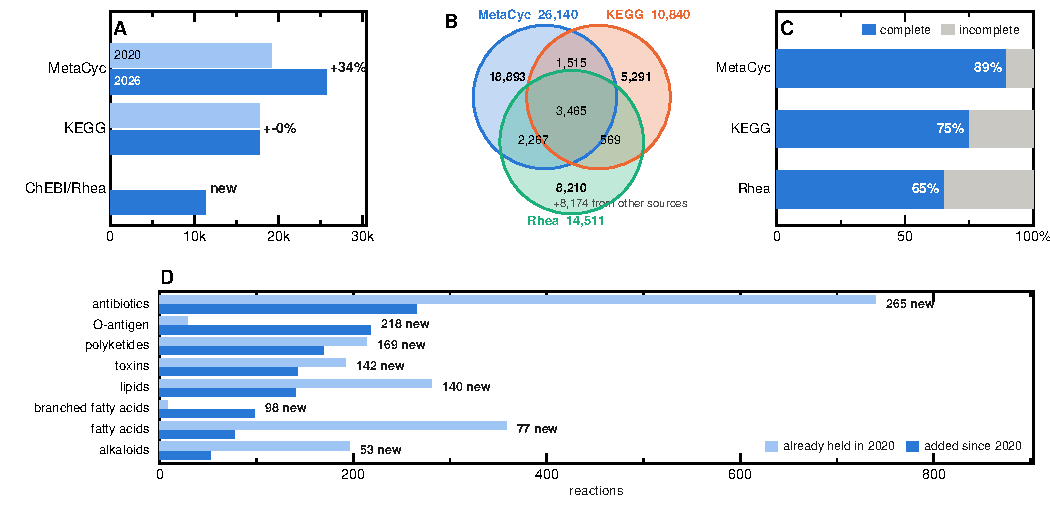
\includegraphics[width=0.88\textwidth]{../figures/figure1_growth.pdf}} %%%
\DIFdelendFL \DIFaddbeginFL \centerline{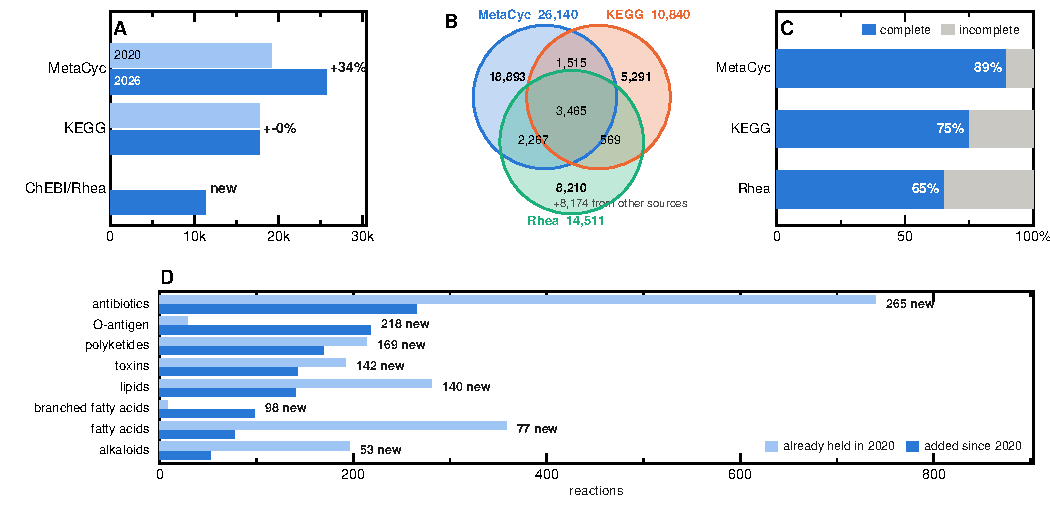
\includegraphics[width=\textwidth]{../figures/figure1_growth.pdf}} \DIFaddendFL \caption{\textbf{Sources of compounds and reactions.} (\textbf{A}) compounds contributed by each source that also supplied molecular structures, 2020 against 2026: we did not introduce any new biochemistry from KEGG\DIFdelbeginFL \DIFdelFL{; }\DIFdelendFL \DIFaddbeginFL \DIFaddFL{. The third row is ChEBI, which supplies structures but no reactions. }\DIFaddendFL (\textbf{B}) \DIFaddbeginFL \DIFaddFL{how }\DIFaddendFL the \DIFdelbeginFL \DIFdelFL{share of each }\DIFdelendFL \DIFaddbeginFL \DIFaddFL{three }\DIFaddendFL primary \DIFdelbeginFL \DIFdelFL{database's reactions that }\DIFdelendFL \DIFaddbeginFL \DIFaddFL{reaction sources overlap, every region labelled with its reaction count. Circle areas }\DIFaddendFL are \DIFdelbeginFL \DIFdelFL{unique; }\DIFdelendFL \DIFaddbeginFL \DIFaddFL{not proportional --- three-set areas cannot be solved exactly --- so the counts carry the quantities and the circles only carry membership. Rhea identifies its compounds through ChEBI. }\DIFaddendFL (\textbf{C}) the share of \DIFdelbeginFL \DIFdelFL{those }\DIFdelendFL \DIFaddbeginFL \DIFaddFL{each source's }\DIFaddendFL unique reactions that are complete, meaning \DIFaddbeginFL \DIFaddFL{every }\DIFaddendFL reagent \DIFdelbeginFL \DIFdelFL{in a reaction }\DIFdelendFL is assigned a complete structure, so the reaction can be balanced and decomposed.\DIFdelbeginFL \DIFdelFL{The three panels share one row per source; the third row is ChEBI in (}\textbf{\DIFdelFL{A}}%DIFAUXCMD
\DIFdelFL{) and Rhea in (}\textbf{\DIFdelFL{B}}%DIFAUXCMD
\DIFdelFL{) and (}\textbf{\DIFdelFL{C}}%DIFAUXCMD
\DIFdelFL{), because ChEBI supplies structures but no reactions and Rhea supplies reactions but no structures. Rhea identifies its compounds through ChEBI, so its completeness is dependent on ChEBI structures.}\DIFdelendFL } \label{fig:growth} \end{figure*}

%% Compact Methods statement for BOTH routes to a direction claim. The full
%% specification of each lives in the supplement:
%%   grading  -> Supplementary Methods S3
%%   ensemble -> Supplementary Methods S4
%% Do not re-expand either here; the budget is 4-6 typeset pages and the detail
%% was moved out deliberately.
\subsection{Grading reaction direction}\label{sec:methods-grading}

We apply a classification approach with which we grade the predicted reaction direction based on the \DIFaddbegin \DIFadd{quality of }\DIFaddend available evidence.
\DIFdelbegin \DIFdel{Very often sources and heuristics disagree, as is the case here, and we qualify what the reaction direction would be, and how reliable the evidence is using several tiers for ease of interpretation: gold }\DIFdelend \DIFaddbegin \DIFadd{The selected tiers are intuitively described as gold (highest), silver (intermediate)}\DIFaddend , \DIFdelbegin \DIFdel{silver, }\DIFdelend or bronze \DIFaddbegin \DIFadd{(lowest)}\DIFaddend .
Our evaluation splits two ways, on the confidence of a source's own claim, fitted as a probability against the experimental anchors, and what the other sources make of it, by a weighted comparison on the same scale.
Grades, self-assessments, and cross-source verdicts are stored in the biochemistry database \DIFdelbegin \DIFdel{, and can be viewed in the UI.
The process of grading reactions is described fully }\DIFdelend \DIFaddbegin \DIFadd{and exposed on the website for users to inspect disagreements among the sources and heuristics for themselves.
The grading methodology is thoroughly described }\DIFaddend in Supplementary Methods~S3.

\subsection{Ensemble LLMs predictions}\label{sec:llm-grading} Thermodynamic assignment is bounded by estimate coverage: energies cannot be computed for an incomplete reaction in terms of structures\DIFdelbegin \DIFdel{. Furthermore, every reaction is a member of a pathway within a cell,and the overarching drive of the pathway, dynamically changing metabolite concentrations as downstream enzymes process reagents, means a reaction may be driven in a direction on a level that supersedes our evaluation~\mbox{%DIFAUXCMD
\cite{mavrovouniotis1993,xu2008,noor2014}}\hskip0pt%DIFAUXCMD
}\DIFdelend \DIFaddbegin \DIFadd{, leaving 23,790 reactions with no direction from any predictor}\DIFaddend . We run a complementary approach using an ensemble, a ``council'' of large language models (LLMs) to interpret the reaction based on its name and stoichiometry alone. Three LLMs independently make their predictions, a fourth audits, and a fifth adjudicates. We provide the prompts in the repository, and describe the process and its limits in Supplementary Methods~S4.
\DIFdelbegin \DIFdel{We integrate these predictions transparently in our database,but do not include them in our grading of the thermodynamic evidence.
}\DIFdelend \DIFaddbegin 

\DIFadd{The ensemble directs 22,963 of the reactions no thermodynamic source will commit on, roughly doubling the fraction of the database that carries a direction. Its accuracy is not that of an energy calculation: scored against measurement it recovers the direction 77\% of the time against 98\% for eQuilibrator, and 85\% of its calls are simply the direction the equation is written in, so its errors fall almost entirely on reactions that run in reverse (Supplementary Methods~S4). We therefore release these calls as a separate, clearly-labelled layer, excluded from the evidence grading: they are for reactions a reconstruction would otherwise leave reversible by default, and should be reviewed before use rather than treated as evidence. Neither approach models the pathway context that can drive a reaction against its own standard-state energy as metabolite concentrations shift downstream~\mbox{%DIFAUXCMD
\cite{mavrovouniotis1993,xu2008,noor2014}}\hskip0pt%DIFAUXCMD
; that remains a property of a model rather than of a reference database.
}

\DIFaddend %% Consolidates the former methods_{reaction_similarity,atom_mapping} sections.
\subsection{Atom mapping}\label{sec:methods-mapping}

Atom mappings are generated from the workflow of Hu{\ss} \textit{et al.}~\cite{huss2022} where they refine the per-reaction output of the Reaction Decoder Tool~\cite{rahman2016} into mappings that can be used to span a metabolic reconstruction.
The approach also resolves chemically equivalent atoms into symmetry groups, such as the two oxygens of CO$_2$ and the six equivalent terminal oxygens of pyrophosphate, so the ambiguity is apparent.
The output is formatted and stored in the database, and can also be visualized in the UI.

%% Consolidates the former methods_{community_ci,distribution} sections.
\subsection{Distribution and community process}\label{sec:methods-distribution}

%% NOT a PyPI package. Corrected 2026-09-07: there is no ModelSEEDDatabase
%% distribution on PyPI (pypi.org/pypi/ModelSEEDDatabase/json returns 404) and
%% this repository carries no packaging config. ModelSEEDpy does exist, but it
%% does not bundle the biochemistry -- it clones this repository and reads it
%% from a local path. Do not reinstate the PyPI claim unless one is published.
The database is distributed as versioned flat files and JSON from the public repository, queried programmatically through a SOLR endpoint, and browsed through the web interface at \modelseedurl.
Every merge runs continuous integration that rebuilds the database from source records and fails on any regression in balance, structure coverage or schema conformance, so a curation change that breaks an invariant cannot be merged.
Researchers \DIFaddbegin \DIFadd{also }\DIFaddend can contribute by adding and curating structures and reactions, \DIFdelbegin \DIFdel{the repository has a guide for doing so, and new data can be merged }\DIFdelend \DIFaddbegin \DIFadd{guidance for which is available in the repository and is managed }\DIFaddend via pull requests.

\section{Results}
%% Table 1 is the only table in the main text; the per-source breakdown that was
%% Table 3 in 2020 moves to Supplementary Table S1.
\subsection{Growth and coverage}\label{sec:results-growth}

The database has grown 34\% in compounds and \DIFdelbegin \DIFdel{55}\DIFdelend \DIFaddbegin \DIFadd{34}\DIFaddend \% in reactions since 2020, \DIFaddbegin \DIFadd{counting only non-obsolete entries at both time points, }\DIFaddend driven mainly by MetaCyc and the BioCyc family. Reaction growth is now split across three primary databases (Figure~\ref{fig:growth}B): MetaCyc carries \DIFdelbegin \DIFdel{31,805 }\DIFdelend \DIFaddbegin \DIFadd{26,140 }\DIFaddend reactions of which \DIFdelbegin \DIFdel{21,258 }\DIFdelend \DIFaddbegin \DIFadd{18,893 }\DIFaddend are supplied by no other primary source, KEGG \DIFdelbegin \DIFdel{14,066 }\DIFdelend \DIFaddbegin \DIFadd{10,840 }\DIFaddend of which 5,\DIFdelbegin \DIFdel{756 }\DIFdelend \DIFaddbegin \DIFadd{291 }\DIFaddend are unique, and the newly-integrated Rhea \DIFdelbegin \DIFdel{17,477 }\DIFdelend \DIFaddbegin \DIFadd{14,511 }\DIFaddend of which 8,\DIFdelbegin \DIFdel{339 }\DIFdelend \DIFaddbegin \DIFadd{210 }\DIFaddend are unique: reactions the database would not otherwise hold. Completeness of reactions differs (Figure~\ref{fig:growth}C). We classify a complete reaction where every reagent can be assigned a complete molecular structure: 90\% of MetaCyc's and \DIFdelbegin \DIFdel{76}\DIFdelend \DIFaddbegin \DIFadd{75}\DIFaddend \% of KEGG's reactions against \DIFdelbegin \DIFdel{66}\DIFdelend \DIFaddbegin \DIFadd{65}\DIFaddend \% of Rhea's. Overall structure coverage rose from 28,\DIFdelbegin \DIFdel{120 }\DIFdelend \DIFaddbegin \DIFadd{087 }\DIFaddend to 36,\DIFdelbegin \DIFdel{943 compounds. }\DIFdelend \DIFaddbegin \DIFadd{907 compounds. The new biochemistry is not distributed like the old (Supplementary Figure~S1): the MetaCyc classes that grew are those of specialised metabolism --- antibiotic and polyketide biosynthesis, O-antigen and cell-envelope assembly, branched and acylated lipids, alkaloids --- while central carbon and energy metabolism account for 41 of the 12,259 reactions added. Central metabolism was already saturated in 2020; what a 2026 reconstruction gains is the periphery. The comparison covers the MetaCyc-sourced additions; Rhea, which supplied 8,409 of the new reactions, has no pathway ontology to place them in.
}

\DIFaddend \subsection{Structure curation}\label{sec:results-structure}

We built and ran our curation pipeline on all structures that would impact the set of roughly 9,000 reactions used in the ModelSEED and PlantSEED reconstruction templates\DIFdelbegin \DIFdel{. }\DIFdelend \DIFaddbegin \DIFadd{, since an error in one of those propagates into every model built from them. This scope reflects a curation priority, not a statement about how much of the database is usable: the templates are discussed in Section~\ref{sec:results-mapping}. }\DIFaddend The conflict pipeline resolved every previously conflicting compound in \DIFdelbegin \DIFdel{three curationrounds. i) Instances where the conflict existed at the level of mobile hydrogens were resolved automatically using historical formula ii) instances where the structures were structurally different were resolved manually iii) instances where resolution was not straight-forward were entered in the }\DIFdelend \DIFaddbegin \DIFadd{a three-staged curation: i) historical formula were used to automatically resolve conflicts in mobile hydrogens; ii) manual curation resolved conflicts in molecular structures; and iii) where steps i-ii fail because of an absence in defensible source formula, reactions were added to a }\DIFaddend mass-balance exclusion registry where we fix an arbitrarily chosen formula\DIFdelbegin \DIFdel{because no source formula was defensible.
}\DIFdelend \DIFaddbegin \DIFadd{.
}

\DIFaddend \begin{figure*}[!t] \centerline{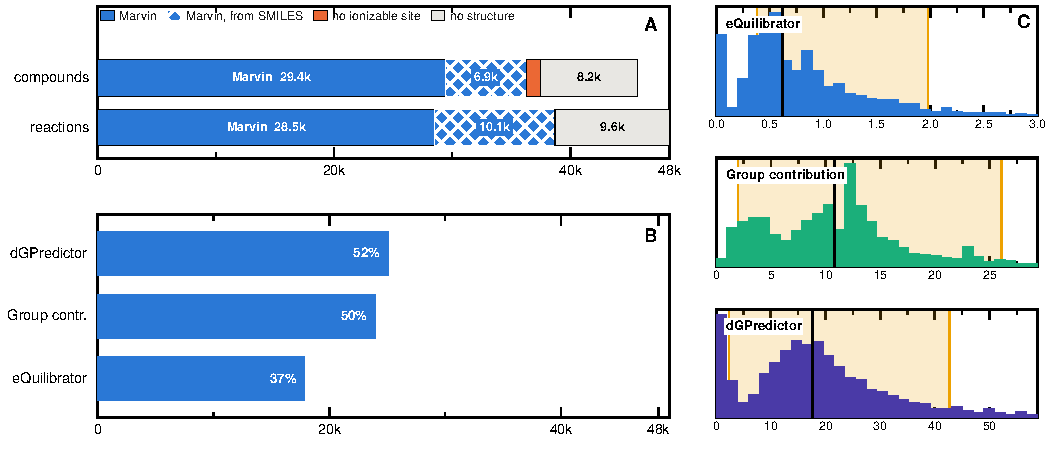
\includegraphics[width=\textwidth]{../figures/figure2_thermodynamics.pdf}} \caption{\textbf{Thermodynamic sources.} (\textbf{A}) Provenance of every pK$_\mathrm{a}$ ladder shipped in the database, across all 45,\DIFdelbeginFL \DIFdelFL{708 }\DIFdelendFL \DIFaddbeginFL \DIFaddFL{662 }\DIFaddendFL compounds and \DIFdelbeginFL \DIFdelFL{56}\DIFdelendFL \DIFaddbeginFL \DIFaddFL{48}\DIFaddendFL ,\DIFdelbeginFL \DIFdelFL{002 }\DIFdelendFL \DIFaddbeginFL \DIFaddFL{384 }\DIFaddendFL reactions. ChemAxon Marvin supplies 79.4\% of compounds and \DIFdelbeginFL \DIFdelFL{81.6}\DIFdelendFL \DIFaddbeginFL \DIFaddFL{79.8}\DIFaddendFL \% of reactions. \DIFaddbeginFL \DIFaddFL{Segments are identified by the key. }\DIFaddendFL \emph{Hatching} marks the share reached through a second route: the calculator refuses polymers and organometallics as query molecules, so those are computed from SMILES instead. \DIFaddbeginFL \emph{\DIFaddFL{No ionizable site}} \DIFaddFL{is a chemistry result --- }\DIFaddendFL Marvin \DIFaddbeginFL \DIFaddFL{ran and }\DIFaddendFL reported no dissociable proton between pH $-2$ and $16$\DIFaddbeginFL \DIFaddFL{, }\DIFaddendFL for 1,\DIFdelbeginFL \DIFdelFL{242 }\DIFdelendFL \DIFaddbeginFL \DIFaddFL{237 }\DIFaddendFL compounds \DIFdelbeginFL \DIFdelFL{. The remainder carry no structure to compute }\DIFdelendFL \DIFaddbeginFL \DIFaddFL{--- and is coloured apart }\DIFaddendFL from \DIFaddbeginFL \emph{\DIFaddFL{no structure}}\DIFaddendFL , which is a curation gap rather than a protonation one. (\textbf{B}) Reactions that carry an energy computed from the source heuristic. (\textbf{C}) Reported uncertainty in kcal\,mol$^{-1}$, one axis per source because the three differ by more than an order of magnitude. The shaded band spans the 5th to 95th percentile, which is used in our classification scheme.} \label{fig:thermo} \end{figure*}

\subsection{Thermodynamics}\label{sec:results-thermo}

%% Counts measured 2026-09-08 from Biochemistry/reaction_*.json after the
%% Marvin 26.1 rebuild. Placeholders excluded per source: group contribution
%% dg = 1e7 (26,555 records); eQuilibrator sigma >= 2500 kcal/mol (3,386),
%% which is that source's refusal marker rather than an error bar.
The three predictors cover comparable fractions of the database and disagree substantially about how well they do it (Figure~\ref{fig:thermo}B). Uncertainty is reported on scales differing by more than an order of magnitude (Figure~\ref{fig:thermo}C): \DIFdelbegin \DIFdel{a median of 0.63\,}\DIFdelend \DIFaddbegin \DIFadd{median errors (}\DIFaddend kcal\,mol$^{-1}$\DIFaddbegin \DIFadd{) of 0.62 for eQuilibrator, 10.83 }\DIFaddend for \DIFdelbegin \DIFdel{eQuilibrator against 10.41\,kcal\,mol$^{-1}$ for }\DIFdelend group contribution\DIFdelbegin \DIFdel{and 17.01\,kcal\,mol$^{-1}$ }\DIFdelend \DIFaddbegin \DIFadd{, and 17.57 }\DIFaddend for dGPredictor.

\paragraph{Calibrating the reported errors against measurement.} We use the experimental anchors to evaluate the error estimates.
For each source\DIFaddbegin \DIFadd{, }\DIFaddend we collect one held-out prediction per anchored reaction, together with the uncertainty that source reports for it, and divide the residual against the measured \drGo{} by that uncertainty.
Measured this way, eQuilibrator has a root mean square of 8.06 and a median of 2.27, with only 28.7\% of reactions within one reported standard deviation and 46.3\% within two, so it understates its error.
Group contribution\DIFdelbegin \DIFdel{runs the other way, with }\DIFdelend \DIFaddbegin \DIFadd{, by contrast, has }\DIFaddend a median of 0.32 and 73.6\% within one standard deviation, and dGPredictor \DIFdelbegin \DIFdel{is the best scaled of the three, }\DIFdelend \DIFaddbegin \DIFadd{performs even better }\DIFaddend with a root mean square of 1.15 and 87.9\% within one \DIFdelbegin \DIFdel{. A researcher choosing by smallest reported error would systematically choose the source that understates it, which is the argument against promoting any single source. }\DIFdelend \DIFaddbegin \DIFadd{standard deviation.
%DIF >  A researcher choosing by smallest reported error would systematically choose the source that understates it, which is the argument against promoting any single source. 
}\DIFaddend The grading in the next section calibrates each source's confidence against measurement rather than taking its uncertainty at face value.

\begin{figure*}[!t]
\centerline{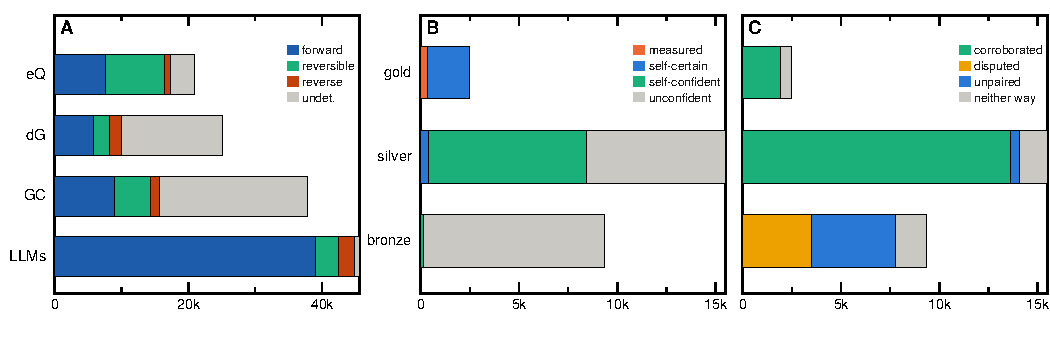
\includegraphics[width=\textwidth]{../figures/figure3_direction.pdf}}
\caption{\DIFdelbeginFL \textbf{\DIFdelFL{Direction, agreement and evidence.}} %DIFAUXCMD
\DIFdelendFL 
        \DIFaddbeginFL \textbf{\DIFaddFL{Direction, agreement, and evidence.}} \DIFaddendFL (\textbf{A}) Direction assigned by each source independently: \emph{eQ} eQuilibrator, \emph{dG} dGPredictor, \emph{GC} group contribution, and \emph{LLMs} the large language model ensemble \DIFdelbeginFL \DIFdelFL{, which supplies a }\DIFdelendFL \DIFaddbeginFL \DIFaddFL{that predicts }\DIFaddendFL direction \DIFdelbeginFL \DIFdelFL{and no }\DIFdelendFL \DIFaddbeginFL \DIFaddFL{but not }\DIFaddendFL energy \DIFdelbeginFL \DIFdelFL{; its calls are released with the database }\DIFdelendFL and \DIFdelbeginFL \DIFdelFL{take no part }\DIFdelendFL \DIFaddbeginFL \DIFaddFL{are not considered }\DIFaddendFL in the evidence grading. Bar length is the number of reactions the source covers, \DIFdelbeginFL \DIFdelFL{so the rows are directly comparable}\DIFdelendFL \DIFaddbeginFL \DIFaddFL{facilitating comparison}\DIFaddendFL . (\textbf{B}) What each evidence grade rests on by the deciding source's own calibrated confidence, and (\textbf{C}) by what the other sources made of it. The two panels share a scale but not a palette, so each carries its own key; categories are ranked as in Supplementary Table~1. \emph{Neither way} is the case that table writes \texttt{---}: a cross-check ran and settled neither way, so it neither helped nor \DIFdelbeginFL \DIFdelFL{penalised}\DIFdelendFL \DIFaddbeginFL \DIFaddFL{penalized}\DIFaddendFL .
    } \label{fig:direction}
\end{figure*}

\subsection{Direction assignment and evidence grading}\label{sec:results-direction}

%DIF < % All direction counts measured 2026-09-08 from Biochemistry/reaction_*.json
%DIF < % after the reversibility overhaul. Grades regenerated the same day against the
%DIF < % Marvin-26.1 energies with
%DIF < %   Scripts/Thermodynamics/SourceGrading/build_tecrdb_comparison.py
%DIF < %   Scripts/Thermodynamics/SourceGrading/grade_thermo_sources.py --cv
%DIF < % Anchors: 797 stereo-exact. The grade tiers are under active revision; the
%DIF < % rates below are for the scheme as it currently ships.
%DIF > % All direction counts re-measured 2026-10-02 from Biochemistry/reaction_*.json
%DIF > % on the live (non-obsolete) population, after promoting the ab33a878 thermo
%DIF > % rerun's reaction_grades.tsv into thermo-evidence/reversibility (previously
%DIF > % unpromoted for 3 days) and re-running grade_thermo_sources.py --cv to drop
%DIF > % 5 reactions physically deleted by 3ac769c1 after ab33a878's snapshot.
%DIF > % Anchors: 801 stereo-exact (438 obsolete duplicates, 363 distinct live).
%DIF > % The grade tiers are under active revision; the rates below are for the
%DIF > % scheme as it currently ships.
Each source now generates its own prediction for the direction each reaction proceeds, and the three sources differ more in what they will commit to than in what they say (Figure~\ref{fig:direction}A). eQuilibrator resolves \DIFdelbegin \DIFdel{84.3}\DIFdelend \DIFaddbegin \DIFadd{97.4}\DIFaddend \% of the reactions it covers, group contribution \DIFdelbegin \DIFdel{42.9}\DIFdelend \DIFaddbegin \DIFadd{59.7}\DIFaddend \% and dGPredictor \DIFdelbegin \DIFdel{41.1}\DIFdelend \DIFaddbegin \DIFadd{40.1}\DIFaddend \%. Across the database, \DIFdelbegin \DIFdel{30,157 }\DIFdelend \DIFaddbegin \DIFadd{24,594 }\DIFaddend reactions receive a direction or a positive statement of reversibility from at least one source and \DIFdelbegin \DIFdel{25,855 }\DIFdelend \DIFaddbegin \DIFadd{23,790 }\DIFaddend receive none.

\paragraph{eQuilibrator vs dGPredictor} dGPredictor is able to generate a predicted energy for more reactions (\DIFdelbegin \DIFdel{$\sim29,600$}\DIFdelend \DIFaddbegin \DIFadd{$\sim25,100$}\DIFaddend , against eQuilibrator's \DIFdelbegin \DIFdel{$\sim21,800$}\DIFdelend \DIFaddbegin \DIFadd{$\sim17,900$}\DIFaddend ) and converts the least of that coverage into a usable reaction direction. For a typical dGPredictor reaction the error bar alone exceeds the decision threshold in the reversibility index, so \DIFdelbegin \DIFdel{58.9}\DIFdelend \DIFaddbegin \DIFadd{59.9}\DIFaddend \% of its reactions are returned undetermined against eQuilibrator's \DIFdelbegin \DIFdel{15.7}\DIFdelend \DIFaddbegin \DIFadd{2.6}\DIFaddend \%. Where both sources commit to a direction they agree \DIFdelbegin \DIFdel{95.0}\DIFdelend \DIFaddbegin \DIFadd{94.8}\DIFaddend \% of the time. dGPredictor is abstaining rather than contradicting, and it resolves \DIFdelbegin \DIFdel{4,248 }\DIFdelend \DIFaddbegin \DIFadd{3,877 }\DIFaddend reactions eQuilibrator cannot, against \DIFdelbegin \DIFdel{13,289 }\DIFdelend \DIFaddbegin \DIFadd{11,237 }\DIFaddend the other way.

\paragraph{Grading.} Of \DIFdelbegin \DIFdel{33,099 }\DIFdelend \DIFaddbegin \DIFadd{27,338 }\DIFaddend graded reactions, \DIFdelbegin \DIFdel{3,434 }\DIFdelend \DIFaddbegin \DIFadd{4,073 }\DIFaddend are gold, \DIFdelbegin \DIFdel{18,388 silver and 11,277 }\DIFdelend \DIFaddbegin \DIFadd{14,475 silver and 8,790 }\DIFaddend bronze (Figure~\ref{fig:direction}\DIFdelbegin \DIFdel{D}\DIFdelend \DIFaddbegin \DIFadd{B,C}\DIFaddend ; see classification scheme in Supplementary Methods~S3). The tiers separate on what supports them: gold is \DIFdelbegin \DIFdel{77}\DIFdelend \DIFaddbegin \DIFadd{91}\DIFaddend \% self-certain and \DIFdelbegin \DIFdel{68}\DIFdelend \DIFaddbegin \DIFadd{85}\DIFaddend \% corroborated, while bronze is 99\% unconfident and split between reactions no second source could check (48\%) and reactions the other sources contradict (\DIFdelbegin \DIFdel{35}\DIFdelend \DIFaddbegin \DIFadd{29}\DIFaddend \%). Because a measured reaction is always graded gold, the grades must be recomputed with openTECR withheld before they can be tested against it. Re-graded on the predictors alone, the \DIFdelbegin \DIFdel{806 anchored reactions split into 357 gold, 437 silver and 12 }\DIFdelend \DIFaddbegin \DIFadd{801 anchored records split into 439 gold, 349 silver and 13 }\DIFaddend bronze; the gold subset falls within 2\,kcal\,mol$^{-1}$ of measurement \DIFdelbegin \DIFdel{96.9}\DIFdelend \DIFaddbegin \DIFadd{93.8}\DIFaddend \% of the time, against \DIFdelbegin \DIFdel{91.3}\DIFdelend \DIFaddbegin \DIFadd{89.4}\DIFaddend \% for silver. \DIFaddbegin \DIFadd{This validation counts records rather than distinct reactions: 438 of the 801 are obsolete duplicates of a live entry, so the effective number of anchored reactions is 363 and these rates rest on fewer independent measurements than the counts imply (Supplementary Methods~S3). }\DIFaddend Both tiers therefore track measurement closely enough that we recommend either for inclusion in a metabolic model, and reserve bronze for review rather than use.

\paragraph{Recommendation.} Evidently where the sources agree on reaction direction, this becomes our recommendation, but because the sources can disagree, we prioritize the source from which we take the recommended reaction direction, so the priority order is eQuilibrator, dGPredictor, group contribution. eQuilibrator supplies \DIFdelbegin \DIFdel{21,218 }\DIFdelend \DIFaddbegin \DIFadd{16,985 }\DIFaddend recommended reaction directions, dGPredictor \DIFdelbegin \DIFdel{4,248 }\DIFdelend \DIFaddbegin \DIFadd{7,935 }\DIFaddend and group contribution \DIFdelbegin \DIFdel{4,691}\DIFdelend \DIFaddbegin \DIFadd{2,055}\DIFaddend ; these numbers include the ones where there is agreement also. We record the source used to make the recommendation, so researchers may apply a different precedence.

%% Consolidates the former results_{atom_mapping,reaction_similarity,
%% connectivity_ontology} sections.
\subsection{Atom mapping}\label{sec:results-mapping}

Atom mappings are published for \DIFdelbegin \DIFdel{32,877 reactions, 59}\DIFdelend \DIFaddbegin \DIFadd{26,242 reactions, 54}\DIFaddend \% of the database: \DIFdelbegin \DIFdel{25,058 }\DIFdelend \DIFaddbegin \DIFadd{19,809 }\DIFaddend clean, and \DIFdelbegin \DIFdel{7,819 }\DIFdelend \DIFaddbegin \DIFadd{6,433 }\DIFaddend that required salvage (which are tagged). As the mappings can be used to span a metabolic reconstruction, reactions needing one repair are likely to carry others.

\DIFaddbegin \paragraph{\DIFadd{Reconstruction scope.}} \DIFadd{A template carries far fewer reactions than the database holds --- the v7.0 ModelSEED templates span 8,597 in union, about 9,000 with PlantSEED\_v3 roles --- but that gap does not mean the remainder is unusable. The database is a reference namespace across all kingdoms and includes biochemistry from secondary databases and published models that no single template targets. Promotion into a template is limited by mass and charge balance, which 69\% of reactions satisfy, and by association to an annotated functional role, which 41\% carry. Gene association is not the constraint: 2,258 of the 8,584 reactions in the Gram-negative template are typed as gapfilling and require no gene. 15,106 reactions now satisfy both balance and role annotation, 8,815 of them outside every current template.
}


\DIFaddend \section{Discussion}

Unlike the 2020 release, this update adopts a multi-source policy rather than promoting a single thermodynamic value, publishing four sources, each with their own uncertainty and estimated direction, because the sources may disagree in ways a single value conceals. Grading against experiment enables us to validate the approach: A researcher can take the highest-graded source and knows what the grade means. \DIFaddbegin \DIFadd{Two limits are worth naming. Transport reactions are scored without a membrane potential or a pH gradient, because both are properties of an organism and a condition rather than of a reference reaction; a compartment-aware scoring layer is the natural next release, and it needs the organism context a model supplies and a database cannot. And roughly half the database still carries no thermodynamic direction at all, bounded by the structures needed to compute one. }\DIFaddend In being explicit about disagreement between sources, we expect this release to serve the widening range of \DIFdelbegin \DIFdel{communities that }\DIFdelend \DIFaddbegin \DIFadd{researchers who }\DIFaddend build on shared biochemistry: genome-scale reconstruction, flux analysis, pathway design and the training of predictive models.
\DIFaddbegin 

\DIFaddend \section{Data availability}

The ModelSEED Biochemistry Database is available at \url{https://github.com/ModelSEED/ModelSEEDDatabase} under the Creative Commons Attribution License, as versioned flat files and JSON, and archived at Zenodo (\url{https://doi.org/10.5281/zenodo.22782602}). Data directly derived from KEGG and MetaCyc remain subject to the licences of those resources. It is also queryable through a Solr endpoint and browsable at \modelseedurl. Released structures, thermodynamic values with per-source uncertainty, evidence grades, atom mappings and the low-confidence reaction flags are all in that repository. The scripts that regenerate every published value, including the eQuilibrator cache rebuild, are under \file{Scripts/Thermodynamics/}.

%% Supplied by Robert Giessmann (2026-09-14), his own wording. Only change:
%% ``wants to acknowledge'' -> ``acknowledges'' for journal register. NAR's
%% Article structure list places Acknowledgements before Author Contributions.
\section{Acknowledgements} R.T.G.\ acknowledges all the hard-working individuals who contributed their time voluntarily to transcribe and check the myriad of numbers and text to create the re-curated openTECR v1.0. The full list of contributors can be found at \url{https://github.com/opentecr}.

%% DRAFT for circulation, not agreed. Role assignment follows Sam's steer of
%% 2026-09-10: Sam lead throughout; Henry conceptualization plus funding and
%% supervision; Freiburger, Faria, Setlur and Taylor major, each supplying part
%% of the resources the release was assembled from; Edirisinghe and Liu minor.
%% External groups are credited for the tool or dataset they contributed.
%% Degrees (lead/equal/supporting) are CRediT's own qualifiers and carry the
%% major/minor distinction without ranking people. Every author must confirm
%% their own line: NAR requires editor approval to change roles after submission.
\section{Author contributions} Contributions follow the CRediT taxonomy. S.M.D.S.: conceptualization, methodology, software, formal analysis, data curation, visualization, writing -- original draft, project administration. C.S.H.: conceptualization, funding acquisition, supervision. A.F., J.P.F., V.S.\ and C.T.: resources, data curation, investigation; J.P.F.\ also writing -- original draft. J.N.E.\ and F.L.: resources, software (supporting). R.T.G.: the openTECR re-curation of the experimental measurements. E.N.\ and M.E.B.: eQuilibrator. V.U., M.A.\ and C.D.M.: dGPredictor. S.H.\ and Z.N.: atom mapping. A.P.A., R.W.C.\ and E.M.W.-C.: funding acquisition, supervision. All authors reviewed the manuscript.

\section{Funding}
%% Sam's wording, 2026-09-07. BRAVE's identifier is as he supplied it.
%%
%% KBase is cited with its FOUR EXTERNAL DOE AWARD NUMBERS, taken from the
%% funding acknowledgement of the most recent KBase paper. An earlier draft of
%% this section used PRJ1003559, which appears in cv.md and 19 times in the
%% mail archive -- but that is an INTERNAL Argonne cost code
%% ("PRJ1003559 66370 Kbase Pred Bio Environ"), not a DOE award number, and it
%% does not belong in a funding statement. Do not reinstate it.
%%
%% DE-AC02-06CH11357 deliberately appears TWICE: once as Argonne's operating
%% contract for this work, and once within KBase's own award list, where it is
%% Argonne's share of the KBase award. That is how KBase states it.
This work was supported by the U.S. Department of Energy, Office of Science, Biological and Environmental Research, under Argonne National Laboratory contract DE-AC02-06CH11357. We specifically acknowledge support from the BRAVE FWP (DOE-112-VAM-PRJ1011481). The DOE Systems Biology Knowledgebase (KBase) is funded by the U.S. Department of Energy, Office of Science, Office of Biological and Environmental Research, under Award Numbers DE-AC02-05CH11231, DE-AC02-06CH11357, DE-AC05-00OR22725, and DE-SC0012704.

\section{Conflict of interest} None declared.

\section{Notice of copyright} The submitted manuscript has been created by UChicago Argonne, LLC, Operator of Argonne National Laboratory (``Argonne''). Argonne, a U.S. Department of Energy Office of Science laboratory, is operated under Contract No.~DE-AC02-06CH11357. The U.S. Government retains for itself, and others acting on its behalf, a paid-up nonexclusive, irrevocable worldwide license in said article to reproduce, prepare derivative works, distribute copies to the public, and perform publicly and display publicly, by or on behalf of the Government. The Department of Energy will provide public access to these results of federally sponsored research in accordance with the DOE Public Access Plan. \url{http://energy.gov/downloads/doe-public-access-plan}


\bibliographystyle{nar}
\bibliography{references}

\end{document}
